\chapter{Evaluation}

\section{Numerical Simulation Results} 

In this section, numerical simulations are conducted to evaluate the correctness of the derived discrete integrators for mechanical models on Lie groups. In particular, the structure-preserving properties of the variational discretizations derived in Section~\ref{sec:} are examined. The analysis focuses especially on the preservation of the momentum map associated with the symmetry of the system, the evolution on the Lie-group configuration manifold, and the long-time behaviour of the total energy. This validation is important since discrete mechanical models obtained by variational integration provide a reliable basis for certifiable trajectory optimization. If the discrete flow violates the manifold structure or introduces artificial drift in conserved quantities such as momentum, the resulting optimization model becomes less faithful to the underlying mechanics \cite{Lee2008}. In contrast, variational integrators are constructed from a discrete variational principle and are symplectic, momentum preserving, and consist robust long-time energy behaviour \cite{Marsden2001}. For the evaluation, the evolution of the total energy, the momentum-map behaviour, and the preservation of the Lie-group structure of the 3D-pendulum are compared with the classical fourth-order Runge-Kutta method and a projected Runge-Kutta on \(SO(3)\) as reference integrators \cite{CELLEDONI2003421, Hairer2000} (see Table. \ref{tab:integrator_comparison}).

\begin{table}[h]
\centering
\caption{Comparison of the considered integration methods properties.}
\label{tab:integrator_comparison}
\begin{tabular}{lcc}
\hline
\textbf{Method} & \textbf{Symplectic} & \textbf{Manifold Preserving} \\
\hline
Variational Integrator & \cmark & \cmark \\
RK4 & \xmark & \xmark \\
Projected RK4 & \xmark & \cmark \\
\hline
\end{tabular}
\end{table}

\paragraph{Runge--Kutta 4th order}
As a basline integrator, the classical explicit fourth-order Runge-Kutta (RK4) is applied to the continuous rigid-body equations written as as first-order system $(\bm{\dot{R}},\bm{\dot{\omega}}) = \bm{f} (\bm{R},\bm{\omega})$. For a system of the form
\begin{align}
    \dot{\bm{y}} = \bm{f}(\bm{y}),
\end{align}
the classical RK4 scheme computes the four stage values
\begin{subequations}\label{eq:rk4_stages}
\begin{align}
    (\bm{k}_1^{R}, \bm{k}_1^{\omega}) &= \bm{f}(\bm{R}_n, \bm{\omega}_n), \\
    (\bm{k}_2^{R}, \bm{k}_2^{\omega}) &= \bm{f}\!\left(\bm{R}_n+\frac{h}{2}\bm{k}_1^R,\bm{\omega}_n+\frac{h}{2}\bm{k}_1^{\omega}\right), \\
    (\bm{k}_3^{R}, \bm{k}_3^{\omega}) &= \bm{f}\!\left(\bm{R}_n+\frac{h}{2}\bm{k}_2^{R},\bm{\omega}_n+\frac{h}{2}\bm{k}_2^{\omega}\right), \\
   (\bm{k}_4^{R}, \bm{k}_4^{\omega}) &= \bm{f}\!\left(\bm{R}_n+h\bm{k}_3^{R}, \bm{\omega}_n+h\bm{k}_3^{\omega}\right),
\end{align}
\end{subequations}
and updates the numerical solution according to
\begin{subequations}\label{eq:rk4_update}
\begin{align}
    \bm{R}_{n+1}
    &=
    \bm{R}_n
    +
    \frac{h}{6}
    \left(
    \bm{k}_1^{R} + 2\bm{k}_2^{R} + 2\bm{k}_3^{R} + \bm{k}_4^{R}
    \right), \\
    \bm{\omega}_{n+1}
    &=
    \bm{\omega}_n
    +
    \frac{h}{6}
    \left(
    \bm{k}_1^{\omega} + 2\bm{k}_2^{\omega} + 2\bm{k}_3^{\omega} + \bm{k}_4^{\omega}
    \right),
\end{align}
\end{subequations}
for each discrete-time step $n$ \cite{butcher2016numerical}.

The explicit RK4 method does not preserve the orthogonality constraint \(\bm{R}^\top \bm{R}=\bm{I}\) and leaves the manifold configuration of $SO(3)$, since the rotation matrix $\bm{R}_n$ is updated additively in the vector space of $\mathbb{R}^{3 \times 3}$ \cite{CELLEDONI2003421}.

\paragraph{RK4 projected to $SO(3)$}

To satisfy the orthogonality constraint 
\[
SO(3)
=
\left\{
\bm{R}\in\mathbb{R}^{3\times 3}
\;\middle|\;
\bm{R}^\top \bm{R}=\bm{I}_3,\ 
\det(\bm{R})=1
\right\}.\]
the explicit RK4 method is combined with a projection of the discrete-time updated rotation matrix $\bm{R}_n$ on $SO(3)$. Therefore, after performing the RK4 step in $\mathbb{R}^{3 \times 3}$ the obtained rotation matrix \(\widetilde{\bm{R}}_{n+1}\), the singular value decomposition is used  
\begin{align}
    \widetilde{\bm{R}}_{n+1}=\bm{U}\bm{\Sigma}\bm{V}^{\top},
\end{align}
following a reconstruction to derive the updated rotation matrix
\begin{align}
    \bm{R}_{n+1}=\bm{U}\bm{V}^{\top},
\end{align}
 which is projected on $SO(3)$ \cite{YanaiTakeuchiTakane2011SVD}. Consequently, $\bm{R}_{n+1}$ satisfy the orthogonality constraint, while the angular velocity $\bm{\omega}_{n+1}$ remains unchanged on the vector space $\mathbb{R}^{3 \times 3}$. However, this method does not inherit structure preserving properties of the Lie group variational integrator, for example, symplecticity or momentum conservation \cite{CELLEDONI2003421}. 

\subsection{3D Pendulum}

For evaluating the geometric properties preservation of the previously defined 3D-pendulum (see Section \ref{sec:discrete_3d_pendulum}), numerical simulations are conducted for the unforced and controlled cases. The rigid body is modeled as a uniform solid cylinder of length $l=\SI{1}{\meter}$ and radius $r=\SI{5}{\cm}$, with its center of mass at $\frac{l}{2}$. Thereby, the physical parameters characterizing the configuration manifold, are chosen as 
\begin{align}
    m &= \SI{1}{\kilogram}, &
    g &= \SI{9.81}{\meter\per\second\squared}, \\
    \bm{\rho}_c &=
    \begin{bmatrix}
        0 & 0 & 0.5
    \end{bmatrix}^\top \si{\meter}, &
    \bm{e}_3 &=
    \begin{bmatrix}
        0 & 0 & 1
    \end{bmatrix}^\top.
\end{align}
 The inertia matrix about the center of mass can be taken from the inertia table given in \cite{RITInertiaTable216}. Here, the rotation of the center of mass in x and y direction are represented about the central diameter $\bm{J}_{11,com}=\bm{J}_{22,com}= \frac{1}{12}m(3r^2 + 4l^2)$, and the rotation of the center of mass in gravity direction z is perpendicular to the axis of rotation $\bm{J}_{33,com}=\frac{1}{2} mr^2$. The off-diagonal terms are equal to zero, because the body-fixed frame is aligned with the principal axes of the cylindrically symmetric body \cite{Lee2008}. Additionally, the inertia matrix about the pivot in body-frame is obtained by the parallel axis theorem of \cite{Benacquista2018ClassicalMechanics} given by
\begin{align}
    \bm{J}
    =
    \bm{J}_{\mathrm{com}}
    +
    m\left(
        \|\bm{\rho}_c\|^2\bm{I}
        -
        \bm{\rho}_c\bm{\rho}_c^{\top}
    \right).
\end{align}
After substituting the chosen values, the 3D-pendulum's inertia matrix is given as
\begin{align}
    \bm{J}
    &=
    \begin{bmatrix}
        0.33396 & 0 & 0 \\
        0 & 0.33396 & 0 \\
        0 & 0 & 0.00125
    \end{bmatrix}
    \si{\kilogram\meter\squared}.
\end{align}
Given \eqref{eq:non-standard_inertia}, the non-standard inertia matrix is calculated to
\begin{align}
    \bm{J}_d
    &=
    \begin{bmatrix}
        0.000625 & 0 & 0 \\
        0 & 0.000625 & 0 \\
        0 & 0 & 0.333333
    \end{bmatrix}
    \si{\kilogram\meter\squared}.
\end{align}
Using the introduced computational approach of Section \ref{sec:discrete_computational_approach}, the derived discrete-time implicit Hamilton equations
of the unforced \eqref{eq:discrete_3D_pendulum_hamilton} and controlled \eqref{eq:forced_3D_pendulum_hamilton} 3D-pendulum are converted to an equivalent vector equation in $\mathbb{R}^3$ using the Cayley transformation. From \cite{ColomboJimenez2012SO3_Cayley}, the corresponding nonlinear vector equation $0 = \bm{A}(\bm{f})$ of the 3D-pendulum is taken as
\begin{equation}\label{eq:simulation_3D_pendulum_vector_equation}
    0 = \bm{a}+\bm{a} \times \bm{f} + \bm{f}(\bm{a}^\top \bm{f})-2 \bm{J} \bm{f} = \bm{A}(f),
\end{equation}
with $\bm{a}= h (\bm{\Pi}_k + \frac{h}{2} \bm{M}_k)$. Additionally, \cite{ColomboJimenez2012SO3_Cayley} defines its Jacobian $\nabla A\!\left(\bm{f}\right)$ to
\begin{align}\label{eq:Caley_Jacobian}
\nabla A(\bm{f})
=
\hat{\bm{a}}
+
(\bm{a}^{\top}\bm{f})\bm{I}
+
\bm{f}\bm{a}^{\top}
-
2\bm{J}.
\end{align}
The tolerance for the Newton iteration is defined to $\left\lVert f^{(i+1)} - f^{(i)} \right\rVert < 10^{-12}$. The initial conditions are taken from \cite{Lee2008} 
\begin{align}
\bm{f}^0 &= (2 \bm{J} - \hat{\bm{a}})^{-1}\bm{a},&
    \bm{R}_0 &= \bm{I}, &
    \bm{\Omega}_0 &=
    \begin{bmatrix}
        4.14 & 4.14 & 4.14
    \end{bmatrix}^{\top}\si{\radian\per\second},
\end{align} where $\bm{f}^0$ is the linearized solution of
\eqref{eq:simulation_3D_pendulum_vector_equation}. The corresponding implementation is documented in the GitHub repository \cite{Elshani2026CTO_GitHub}.

\subsubsection{Unforced 3D-Pendulum}

\begin{figure}[t]
    \centering
    \begin{minipage}{0.48\textwidth}
        \centering
        
\includegraphics[width=\textwidth]{pics/Numerical_Simulation/Total_Energy.pdf}
        \caption*{(a) Total energy $E_k$.}
    \end{minipage}
    \hfill
    \begin{minipage}{0.48\textwidth}
        \centering
        
\includegraphics[width=\textwidth]{pics/Numerical_Simulation/Delta_E.pdf}
        \caption*{(b) Energy deviation $\Delta E_k$.}
    \end{minipage}

    \vspace{0.5em}

    \begin{minipage}{0.48\textwidth}
        \centering
        
\includegraphics[width=\textwidth]{pics/Numerical_Simulation/Momentum_error.pdf}
        \caption*{(c) Momentum error $\Delta \mu_k$.}
    \end{minipage}
    \hfill
    \begin{minipage}{0.48\textwidth}
        \centering
        
\includegraphics[width=\textwidth]{pics/Numerical_Simulation/Orthogonality_error.pdf}
        \caption*{(d) Orthogonality error $e_{orth}$.}
    \end{minipage}

    \caption{Comparison of the numerical preservation properties for the unforced $3$D pendulum.}
    \label{fig:simulation_results_3d_pendulum}
\end{figure}

The results of the numerical simulation for the unforced case, with 
$\bm{u}_k=\bm{0}$, are shown in Fig.~\ref{fig:simulation_results_3d_pendulum}. 
The simulation is performed over $1000$ discrete-time steps with a step size of 
$h=\SI{0.05}{\second}$. Thereby, the accuracy of the different integrator methods, given in Table \ref{tab:integrator_comparison}, are compared to each other, by plotting the corresponding total energy
\[
 E_k
    =
    \frac{1}{2}\bm{\Omega}_k^{\top}\bm{J}\bm{\Omega}_k
    -
    mg\,\bm{e}_3^{\top}\bm{R}_k\bm{\rho}_c,
\]
and its deviation $\Delta E_k = E_k - E_0$, the angular momentum error along the gravity direction
\[
\Delta \mu_k= \bm{e}_3^{\top}\bm{R}_k\bm{\Pi}_k - \bm{e}_3^{\top}\bm{R}_0\bm{\Pi}_0,
\]
defined in \cite{Lee2008}, and the orthogonality error 
\[
e_{\mathrm{orth},k} = \left\|\bm{I}-\bm{R}_k^{\top}\bm{R}_k\right\|_F.
\]

The total energy (see Fig. \ref{fig:simulation_results_3d_pendulum} (a)) and the corresponding energy deviation (see Fig. \ref{fig:simulation_results_3d_pendulum} (b)) illustrates the preserving energy behavior over a long-time in discrete-time flow for the Lie Group Variational Integrator (LGVI). It remains close to the reference level with only small bounded oscillations, because of their symplectic strcuture, which are the exact solution of a pertubed Hamiltonian \cite{Hairer1994}. However, the RK4 and projected RK4 display a clear drift of the energy away from its real value, which remains constant for this model, as the system is unforced.

Moreover, the momentum error (see Fig. \ref{fig:simulation_results_3d_pendulum} (c)) confirms that the LGVI method preserves the momentum, validated for continuous time in \ref{sec:continuous_3D_pendulum_momentum_validation}. The computational results of RK4 and its projection on $SO(3)$ show that these methods are not reliable drifting from the momentum initial value, as they not preserve the total linear momentum \cite{Lee2008}. Especially, the projected RK4 consists of a stronger discrepancy, as it fixes $\bm{R}^\top\bm{R} = \bm{I}$, while the angular velocity $\bm{\omega}$ remains unchanged, which influences the momentum.

Lastly, the orthogonality error highlights that the structure of the Lie group configuration manifold is well preserved in the LGVI, which is depictured in Fig. \ref{fig:simulation_results_3d_pendulum} (d). Similar result is obtained from the projected RK4, while the classic explicit RK4 violates the orthogonality constraint. For RK4 $e_{orth}$ increases linearly with respect to the simulation time-steps.

Consequently, only the LGVI preserves the manifold structure together with the momentum and energy behaviour over a long-time horizon. While RK4 can be projected to the Lie group manifold of $SO(3)$, it can not preserve the momentum and consists of drifting energy behaviour over long-time.

\subsubsection{Controlled 3D-Pendulum}

In the controlled case, the previously derived free dynamics of the 3D-pendulum
are extended by an external body-fixed control moment. Following defined control
structure of \eqref{eq:external_control_moment_3D_pendulum}, the time-dependent control parameter is chosen as
\begin{align}
    \label{eq:controlled_3d_pendulum_input_parameter}
    \bm{u}_p(t)
    =
    \begin{bmatrix}
        0.15\sin(0.5t) \\
        0.10\cos(0.25t) \\
        0
    \end{bmatrix}.
\end{align}
The corresponding discrete control input is obtained by evaluating the control law
at the discrete time nodes $\bm{u}_{p,k} =\bm{u}_p(t_k)$. Thus, the control input acts as a body-fixed external moment that is orthogonal to
the gravity direction expressed in the body frame, given by
$\bm{R}_k^{\top}\bm{e}_3$. Consequently, the control moment has no component
along this direction.

For the RK4 simulation, the continuous-time Hamilton equations \eqref{eq:continuous_3D_pendulum_hamilton} are used, 
adding the contol input $\bm{u(t)}$, based on Lagrange-d' Alembert principle of Section \ref{sec:discrete_forced_lagrangian}.
With the body angular momentum defined by $\bm{\Pi} = \bm{J}\bm{\Omega}$,
the forced continuous-time equations of motion are written as
\begin{subequations}
\label{eq:controlled_3d_pendulum_continuous_RK4}
\begin{align}
    \dot{\bm{\Pi}}
    &=
    mg\,\bm{\rho}_c
    \times
    \bm{R}^{\top}\bm{e}_3
    -
    \bm{J}^{-1}\bm{\Pi}
    \times
    \bm{\Pi}
    +
    \bm{u}(t),
    \label{eq:controlled_3d_pendulum_continuous_momentum}
    \\
    \dot{\bm{R}}
    &=
    \bm{R}
    \left(
        \bm{J}^{-1}\bm{\Pi}
    \right)^{\wedge}.
    \label{eq:controlled_3d_pendulum_continuous_kinematics}
\end{align}
\end{subequations}
In contrast to the unforced case, the external input acts on the system.
Therefore, the total energy and the momentum map are no longer expected to be
conserved.

For the Lie group variational integrator, the forced discrete Hamilton equations
derived in \eqref{eq:forced_3D_pendulum_hamilton} are applied. The implicit
equation for the relative update $\bm{F}_k$ is again solved by using the Cayley
transformation. Compared to the unforced case, only the vector
$\bm{a}$ in \eqref{eq:simulation_3D_pendulum_vector_equation} changes due to
the additional control input. For the controlled dynamics, it is given by
\begin{align}
    \label{eq:controlled_3d_pendulum_cayley_a}
    \bm{a}
    =
    h
    \left(
        \bm{\Pi}_k
        +
        \frac{h}{2}
        \left(
            \bm{M}_k+\bm{u}_k
        \right)
    \right).
\end{align}
Therefore, the nonlinear vector equation \eqref{eq:simulation_3D_pendulum_vector_equation}
and its Jacobian \eqref{eq:Caley_Jacobian} are solved equaly for the unforced simulation, with
the modified vector $\bm{a}$ including the control contribution. After computing
$\bm{f}_k$, the relative attitude update is obtained from the Cayley transformation
and the discrete-time states are propagated according to the forced LGVI. The corresponding implementation
is documented in the GitHub repository \cite{Elshani2026CTO_GitHub}

The numerical simulation of the controlled 3D-pendulum compares the classical RK4 method with the forced
LGVI. Since the purpose of this experiment is to evaluate the behaviour of the
forced variational discretization under an external input, the projected RK4 method
is not considered in this comparison. The same physical parameters and initial
conditions as in the unforced case are used.

Fig.~\ref{fig:forced_3d_pendulum_results} shows the numerical results for the
controlled 3D-pendulum. The simulation is performed over $N=100$ discrete-time
steps with step size $h=\SI{0.001}{\second}$. This shorter time interval is chosen
because the differences between the RK4 method and the forced LGVI already become
visible after a small number of time steps. During approximately the first eight
time steps, both methods show almost identical behaviour, which indicates that the
derived forced equations and their implementation are consistent. As the simulation
progresses, however, the trajectories begin to separate.

\begin{figure}[t]
    \centering
    \begin{minipage}{0.48\textwidth}
        \centering
        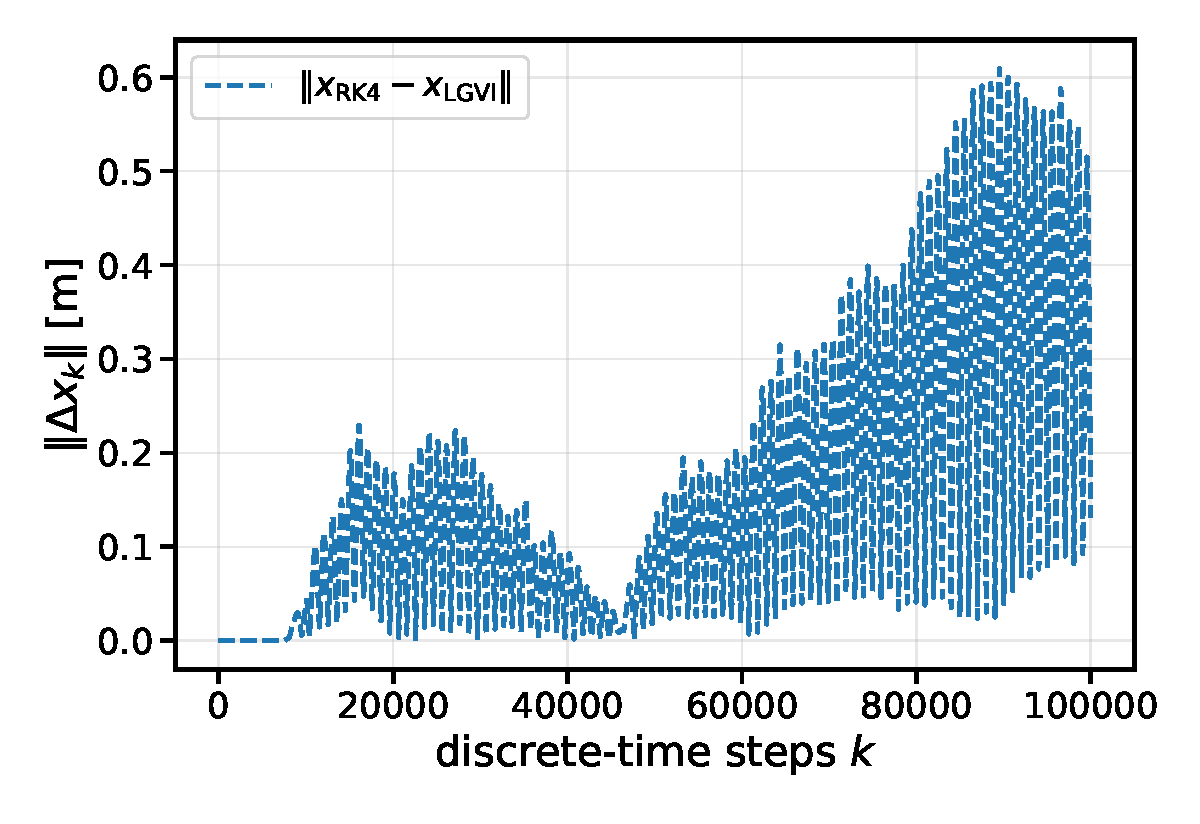
\includegraphics[width=\textwidth]{pics/Numerical_Simulation/Forced_3D_Pendulum_Trajectory.pdf}
        \caption*{(a) Position error norm $\|\Delta \bm{x}_k \||$.}
    \end{minipage}
    \hfill
    \begin{minipage}{0.48\textwidth}
        \centering
        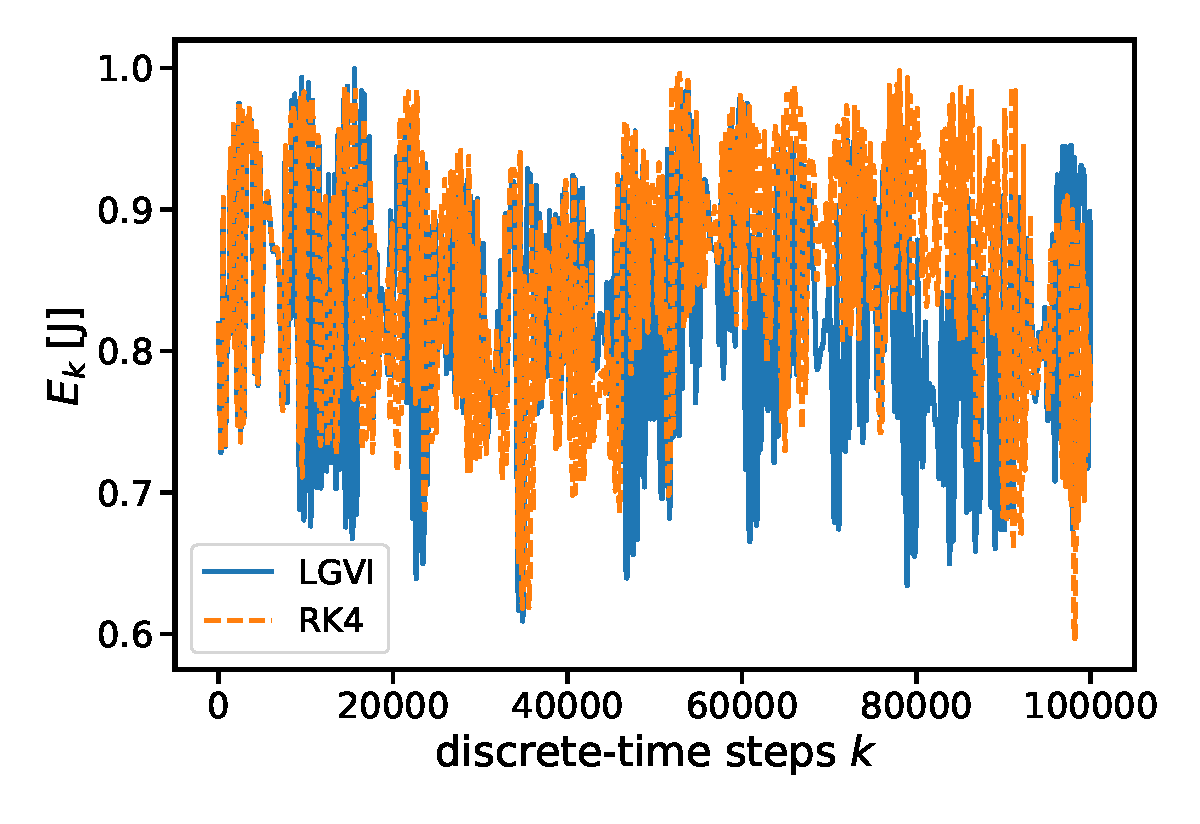
\includegraphics[width=\textwidth]{pics/Numerical_Simulation/Forced_3D_Pendulum_Ek.pdf}
        \caption*{(b) Total energy $E_k$.}
    \end{minipage}

    \vspace{0.5em}

    \begin{minipage}{0.48\textwidth}
        \centering
        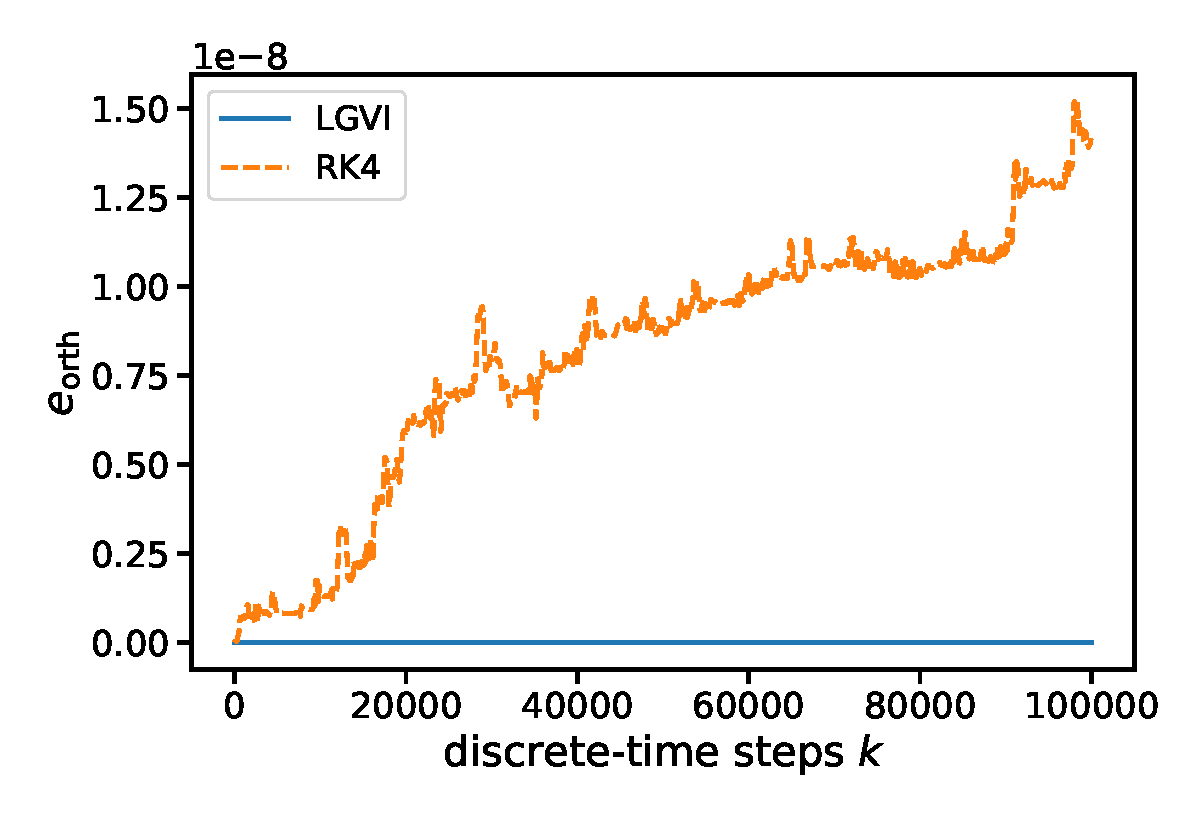
\includegraphics[width=\textwidth]{pics/Numerical_Simulation/Forced_3D_Pendulum_Orth_Error.pdf}
        \caption*{(c) Orthogonality error $e_{\mathrm{orth},k}$.}
    \end{minipage}
    \hfill
    \begin{minipage}{0.48\textwidth}
        \centering
        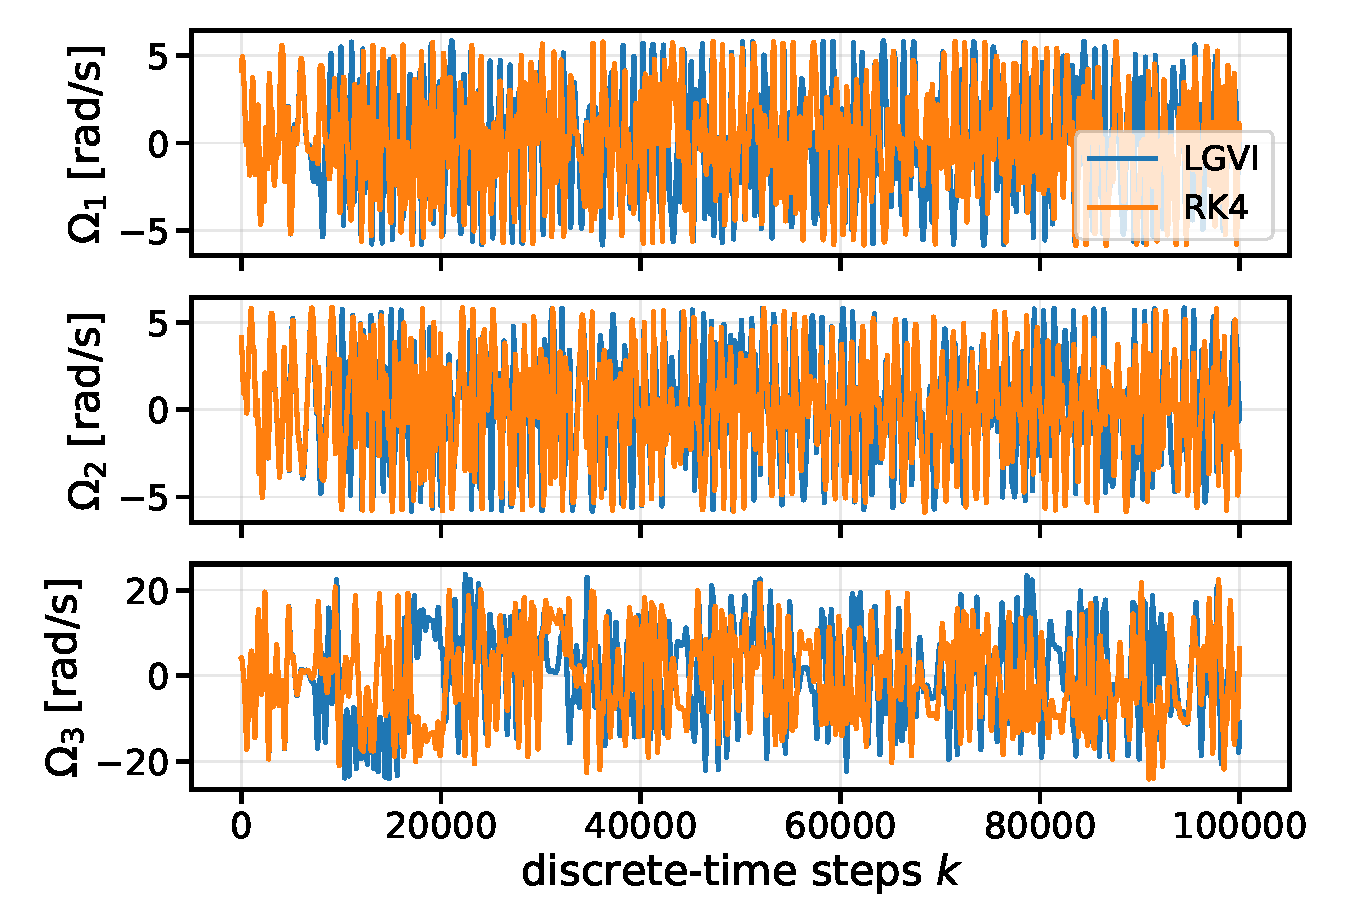
\includegraphics[width=\textwidth]{pics/Numerical_Simulation/Forced_3D_Pendulum_Omega.pdf}
        \caption*{(d) Angular velocity components $\bm{\Omega}_k$.}
    \end{minipage}

    \caption{Comparison of the forced LGVI and RK4 simulation for the controlled $3$D pendulum.}
    \label{fig:forced_3d_pendulum_results}
\end{figure}

The position error in Fig.~\ref{fig:forced_3d_pendulum_results}~(a) is computed
from the center-of-mass position $\bm{x}_k=\bm{R}_k\bm{\rho}_c$,
as
\begin{align}
    \Delta \bm{x}_k
    =
    \left\|
        \bm{x}_{k,\mathrm{RK4}}
        -
        \bm{x}_{k,\mathrm{LGVI}}
    \right\|_2 .
\end{align}
The plot shows that the position error $\Delta \bm{x}_k$ is initially close to zero, but increases
over the simulation. Therefore, both methods reproduce the same short-time motion,
while their trajectories separate after a certain number of time steps. This behaviour is
expected for forced rigid-body dynamics, where small numerical
differences in the attitude $\bm{R}_k$ and momentum update $\bm{\Pi}_k$ can accumulate over time.

The total energy is shown in Fig.~\ref{fig:forced_3d_pendulum_results}~(b).
In contrast to the unforced case, the total mechanical energy is not expected to be
conserved, since the external input $u_{p,k}$ acts on the system. It is observed that
energetic behaviour of LGVI and RK4 under the same applied control
input follow a similar trend at the beginning, but small deviations
appear as the trajectories begin to separate, which is consistent with the position error.

The orthogonality error $e_{\mathrm{orth},k}$ is illustrated in Fig.~\ref{fig:forced_3d_pendulum_results}~(c).
Again, the plot confirms that the LGVI preserves the Lie group structure staying on the manifold by updating the attitude through
$\bm{R}_{k+1}=\bm{R}_k\bm{F}_k$ with $\bm{F}_k\in SO(3)$. For RK4, the attitude is
updated additively in the surrounding vector space using the discrete update map \eqref{eq:rk4_update}. Over the short interval and due
to the small step size $h$, the orthogonality error remains small, but it is not preserved and increased over time, especially for a long time horizon and smaller step sizes $h$.

Finally, Fig.~\ref{fig:forced_3d_pendulum_results}~(d) compares the angular
velocity components $\bm{\Omega}_k$. In the discrete Hamiltonian formulation, the angular velocity
is recovered from the body angular momentum by
\begin{align}
    \hat{\bm{\Omega}}_k
    =
    (\bm{J}^{-1}\bm{\Pi}_k)^\wedge,
\end{align}
discretizing and solving \eqref{eq:continuous_3D_pendulum_momentum} for $\hat{\bm{\Omega}}_k$.
The angular velocity components of LGVI and RK4 are equal at the beginning of the
simulation, but begin to differ after a small number of steps. This confirms the
same behaviour observed in the position error $\Delta \bm{x}_k$ and the ploted Energy $E_k$.
The 3D-Pendulum numerical simulation using external control inputs produces
consistent short-time dynamics of LGVI and RK4, while the numerical trajectories between both methods separate as the
simulation continues.

\subsection{Acrobot}
\label{subsec:evaluation_acrobot}

TODO: bm all vectors and matrices also simplify and explain Cayley transformation used

To evaluate the geometric properties preservation of the previously defined Acrobot (see Section \ref{sec:acrobot}), 
numerical simulations are conducted for the unforced and controlled case similar to those conducted for the 3D-pendulum 
in Section \ref{sec:numerical_simulation_3d_pendulum}.
In contrast to the 3D-pendulum, the Acrobot is a constrained multi-body system in maximal coordinates with the configuration 
\[
\bm{q}_k =
\left(
\bm{x}_{1,k},
\bm{R}_{1,k},
\bm{x}_{2,k},
\bm{R}_{2,k}
\right)
\in
\left(\mathbb{R}^{2}\times SO(2)\right)^2 ,
\]
Therefore, the validation does not only focus on the preservation of the Lie-group structure of the attitude variables, but also on the preservation of the holonomic joint constraints $\bm{\phi}_0(\bm{q}_k)$ and $\bm{\phi}_{12}(\bm{q}_k)$. 
The physical parameters are chosen as two identical uniform rods with
\[
    m_1=m_2=1\,\mathrm{kg},
    \qquad
    l_1=l_2=0.5\,\mathrm{m},
    \qquad
    g=9.81\,\mathrm{m/s^2},
\]
and the center of mass of each link is located at $\frac{l_i}{2}$.
Since the maximal-coordinate formulation already represents the translational
motion of the link centers of mass, the rotational inertia is taken about the
corresponding center of mass. \cite{Benacquista2018ClassicalMechanics} defines
the rotational inertia of a uniform rod about its center of mass as
\[
    J_i^{\mathrm{com}}
    =
    \frac{1}{12}m_i l_i^2.
\]
The defined non-standard inertia matrix in \ref{eq:non-standard_inertia}
is valid for $SO(3)$. Therefore, the planar
\(SO(2)\) rotational kinetic term of the discrete Lagrangian in
\cite{LeeLeokMcClamroch2007DiscreteControlSystems} is rewritten, which gives the relation of a planar non-standard
inertia to the standard inertia as
\begin{align}\label{eq:2D_nonstandard_inertia}
    J_{d,i}
    =
    \frac{1}{2}J_i^{\mathrm{com}} I_2.
\end{align}
Therefore, the discrete-time inertia matrices of both links are
\[
    J_{d,1}
    =
    J_{d,2}
    =
    \begin{bmatrix}
        0.0104167 & 0\\
        0 & 0.0104167
    \end{bmatrix}
    \mathrm{kg\,m^2},
\]
substituting the chosen values of $m_i$ and $l_i$ into \eqref{eq:2D_nonstandard_inertia}.
The base point is fixed at
\[
    \bm{p}_0 =
    \begin{bmatrix}
        0 & 0
    \end{bmatrix}^{\top}.
\]
Using the body-fixed link convention from Section 4.3.1, the joint vectors are
\[
\rho_{1,0}
=
\begin{bmatrix}
0 & 0.25
\end{bmatrix}^{\top}\mathrm{m},
\qquad
\rho_{1,12}
=
\begin{bmatrix}
0 & -0.25
\end{bmatrix}^{\top}\mathrm{m},
\qquad
\rho_{2,12}
=
\begin{bmatrix}
0 & 0.25
\end{bmatrix}^{\top}\mathrm{m},
\]
illustrated in Fig. \ref{fig:acrobot_maximal_coordinates}.

As in the controlled 3D-pendulum simulation, the classical RK4 method is used as a reference method. However, the projected RK4 method from the unforced 3D-pendulum comparison is not used for the Acrobot. Although a projection based on the singular value decomposition can enforce the orthogonality condition after each RK4 step, the resulting method is not derived from a discrete variational principle. Therefore, it does not automatically inherit the symplectic and momentum-preserving properties of variational integrators \cite{Marsden2001,CELLEDONI2003421,Hairer2000}. Moreover, the projection modifies the numerical flow after the RK4 update. This can influence dynamical quantities such as momentum and energy, as already observed in the 3D-pendulum simulation. Consequently, for the Acrobot, the RK4 reference is integrated in relative coordinates and reconstructed into maximal coordinates. This is a more meaningful comparison, since the relative-coordinate RK4 trajectory satisfies the joint geometry by construction, while the LGVI directly enforces the holonomic constraints in maximal coordinates.

The following metrics are used for the Acrobot simulation. The total mechanical energy is evaluated as
\[
E_k
=
\frac{1}{2}v_{1,k}^{\top}M_1v_{1,k}
+
\frac{1}{2}v_{2,k}^{\top}M_2v_{2,k}
+
\frac{1}{2}J_1\omega_{1,k}^{2}
+
\frac{1}{2}J_2\omega_{2,k}^{2}
+
g e_2^{\top}M_1x_{1,k}
+
g e_2^{\top}M_2x_{2,k},
\]
where $e_2=[0\;1]^{\top}$ denotes the vertical direction. The position difference between the LGVI trajectory and the reconstructed RK4 reference trajectory is computed by
\[
\Delta x_k
=
\left\|
X_{k,\mathrm{RK4}}
-
X_{k,\mathrm{LGVI}}
\right\|_2,
\]
with
\[
X_k =
\begin{bmatrix}
x_{1,k}^{\top} & x_{2,k}^{\top}
\end{bmatrix}^{\top}.
\]
The holonomic constraint residuals are evaluated separately as
\[
\|\bm{\phi}_{0,k}\|_2,
\qquad
\|\bm{\phi}_{12,k}\|_2,
\]
where $\bm{\phi}_{0,k}$ denotes the fixed-base constraint and $\bm{\phi}_{12,k}$ denotes the elbow constraint. Finally, the Lie-group preservation of both link attitudes is measured by
\[
e_{\mathrm{orth},i,k}
=
\left|
I_2 - R_{i,k}^{\top}R_{i,k}
\right|_F,
\qquad
i\in{1,2}.
\]
In contrast to the 3D-pendulum, no momentum-map error is evaluated for the Acrobot. Due to the fixed base joint and the holonomic coupling between the links, the system does not have the same rotational symmetry about the gravity direction as the 3D-pendulum. Therefore, the holonomic constraint residuals are the more relevant structure-preservation metric for the constrained multi-body system.

\subsubsection{Unforced Acrobot}

The first Acrobot simulation considers the unforced case with $u_k=0$. The simulation is performed with the step size
\[
h=\SI{0.1}{\second}
\]
over the final time
\[
t_f=\SI{10000}{\second},
\]
which corresponds to $N=100000$ discrete-time steps. The purpose of this experiment is to evaluate the long-time qualitative behaviour of the maximal-coordinate LGVI and to compare it with the RK4 reference trajectory. In addition, the implementation also computes an RK4 trajectory in maximal coordinates with acceleration-level constraints. This trajectory is used as an additional diagnostic for constraint drift, since acceleration-level constraints enforce $\ddot{\phi}=0$, but do not project the position-level constraint $\phi=0$. The plots in Fig.~6.3 focus on the comparison between the maximal-coordinate LGVI and the relative-coordinate RK4 reference.

The total energy evolution is shown in Fig.~6.3(a). Since the system is unforced, the exact mechanical energy is expected to remain constant. The LGVI energy remains close to its initial value and shows bounded oscillations over the long-time horizon. This behaviour is consistent with the symplectic structure of variational integrators, which generally leads to good long-time energy behaviour instead of monotonic numerical drift. In contrast, the RK4 reference shows a visible drift of the energy over time. This agrees with the observation from the unforced 3D-pendulum simulation in Fig.~6.1, where the LGVI preserved the qualitative energy behaviour more reliably than the classical RK4 method.

Fig.~6.3(b) shows the position error norm $\|\Delta x_k\|$ between the LGVI trajectory and the reconstructed RK4 reference. At the beginning of the simulation, both methods produce similar trajectories. Over the long-time horizon, however, small differences in the numerical integration accumulate and lead to a visible separation of the center-of-mass trajectories. The error remains oscillatory, which is expected for the coupled pendulum-like motion of the Acrobot. Therefore, the plot does not indicate a violation of the constraints, but rather the long-time separation of two different numerical discretizations.

The holonomic constraint residuals are shown in Fig.~6.3(c). Both the base constraint residual $\|\phi_{0,k}\|_2$ and the elbow constraint residual $\|\phi_{12,k}\|_2$ remain close to machine precision over the complete simulation. This confirms that the constrained LGVI enforces the fixed-base joint and the elbow joint at the position level. This result is particularly important for the Acrobot, since the constraints define the physical two-link mechanism. If the constraints were not preserved, the maximal-coordinate states would no longer represent a valid Acrobot configuration.

Finally, Fig.~6.3(d) shows the orthogonality error of both link rotations. The LGVI preserves the $SO(2)$ structure of both attitudes by the multiplicative update $R_{i,k+1}=R_{i,k}F_{i,k}$ with $F_{i,k}\in SO(2)$. The RK4 reference also remains close to machine precision in this plot, because it is integrated in relative coordinates and then reconstructed into rotation matrices. Hence, the RK4 curve should not be interpreted as an additive matrix RK4 method on $SO(2)$. The main differences between both approaches are instead the energy behaviour and the direct preservation of the holonomic constraints in maximal coordinates.

Overall, the unforced Acrobot simulation confirms that the derived constrained LGVI preserves the geometric structure of the maximal-coordinate model. The link attitudes remain on $SO(2)$, the joint constraints remain satisfied, and the energy shows bounded long-time behaviour. This validates the unforced Acrobot discretization derived in Section~4.3.1.

\subsubsection{Controlled Acrobot}

In the controlled case, the Acrobot is actuated by a scalar torque at the elbow joint. As derived in Section~4.3.1, this torque is an internal joint torque acting between the two links. Therefore, it enters the absolute-link virtual work as
\[
\tau_k
=
\begin{bmatrix}
-u_k \\
u_k
\end{bmatrix}.
\]
The control input is chosen as the sinusoidal elbow torque
\[
u(t):=0.15\sin(0.7t)\,\si{\newton\meter}.
\]
The discrete input is obtained by evaluating the continuous input at the time nodes, $u_k=u(t_k)$. The forced simulation uses the same physical parameters and initial condition as the unforced case. The simulation is performed with
\[
h=\SI{0.001}{\second},
\qquad
t_f=\SI{100}{\second},
\]
which again corresponds to (N=100000) discrete-time steps. The same metrics as in the unforced case are evaluated. However, the total mechanical energy is no longer expected to be conserved, since the elbow motor performs work on the system.

The total energy of the controlled Acrobot is shown in Fig.~6.4(a). In contrast to the unforced simulation, the applied torque changes the mechanical energy of the system. Therefore, the relevant observation is not conservation of $E_k$, but the consistency between the LGVI and RK4 energy evolution under the same control input. Both methods show a similar energy behaviour with small oscillations caused by the sinusoidal actuation. This indicates that the forced discrete Lagrange--d'Alembert contribution has been implemented consistently.

Fig.~6.4(b) shows the position error norm $\|\Delta x_k\|$ between the LGVI trajectory and the reconstructed RK4 reference. Compared to the unforced long-time simulation, the error remains significantly smaller over the considered horizon. The difference grows slowly, but stays several orders of magnitude below the link length scale. This confirms that the forced maximal-coordinate LGVI and the relative-coordinate RK4 reference produce nearly identical short-time dynamics under the sinusoidal elbow input. The remaining difference is expected, since the two methods discretize the dynamics differently.

The holonomic constraint residuals are plotted in Fig.~6.4(c). The base and elbow constraint residuals remain close to numerical precision over the complete simulation. Hence, also in the forced case, the maximal-coordinate LGVI prevents constraint drift and keeps the Acrobot links physically connected. This is essential for the later SDP formulation, since the polynomial equality constraints in the optimization problem are based on the same fixed-base and elbow-joint equations.

Finally, Fig.~6.4(d) shows the orthogonality error of both link rotations. As in the unforced simulation, the LGVI preserves the $SO(2)$ structure through the multiplicative attitude update. The reconstructed RK4 reference also remains close to machine precision, since its rotations are computed from relative angles. Therefore, the controlled Acrobot simulation confirms that both the forcing term and the constrained Lie-group update are numerically consistent.

In summary, the Acrobot results in Fig.~6.3 and Fig.~6.4 extend the numerical validation from the single rigid-body 3D pendulum to a constrained multi-body system. The LGVI preserves the $SO(2)$ attitude structure, enforces the holonomic constraints, and shows stable long-time energy behaviour in the unforced case. Under sinusoidal actuation, the forced LGVI remains consistent with the RK4 reference while maintaining the constraint manifold. Therefore, the numerical simulations support the correctness of the derived Acrobot variational integrator and its use as the dynamics model for the optimization formulation in Section~5.3.2.


\begin{figure}[t]
    \centering
    \begin{minipage}{0.48\textwidth}
        \centering
        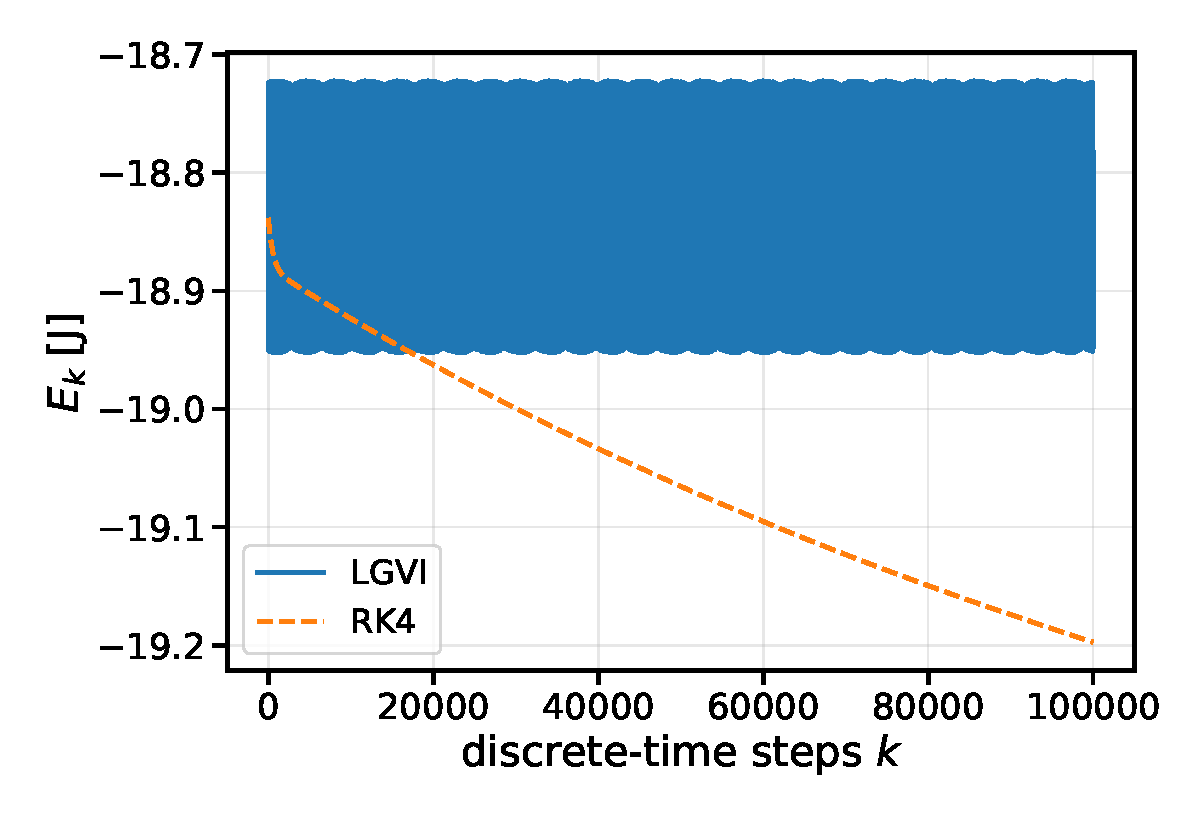
\includegraphics[width=\textwidth]{pics/Numerical_Simulation/Acrobot/acrobot_unforced_total_energy.pdf}
        \caption*{(a) Total energy $E_k$.}
    \end{minipage}
    \hfill
    \begin{minipage}{0.48\textwidth}
        \centering
        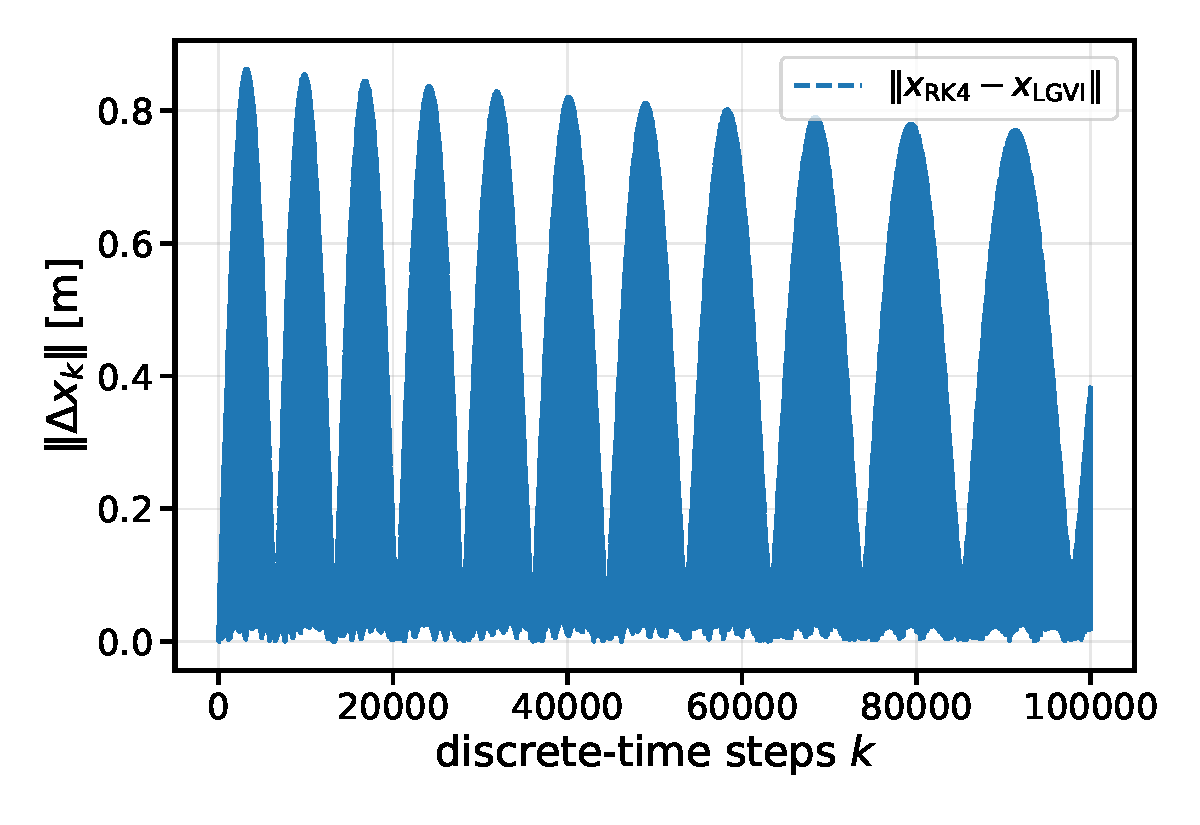
\includegraphics[width=\textwidth]{pics/Numerical_Simulation/Acrobot/acrobot_unforced_position_error_norm.pdf}
        \caption*{(b) Position error norm $\|\Delta \bm{x}_k \||$.}
    \end{minipage}

    \vspace{0.5em}

    \begin{minipage}{0.48\textwidth}
        \centering
        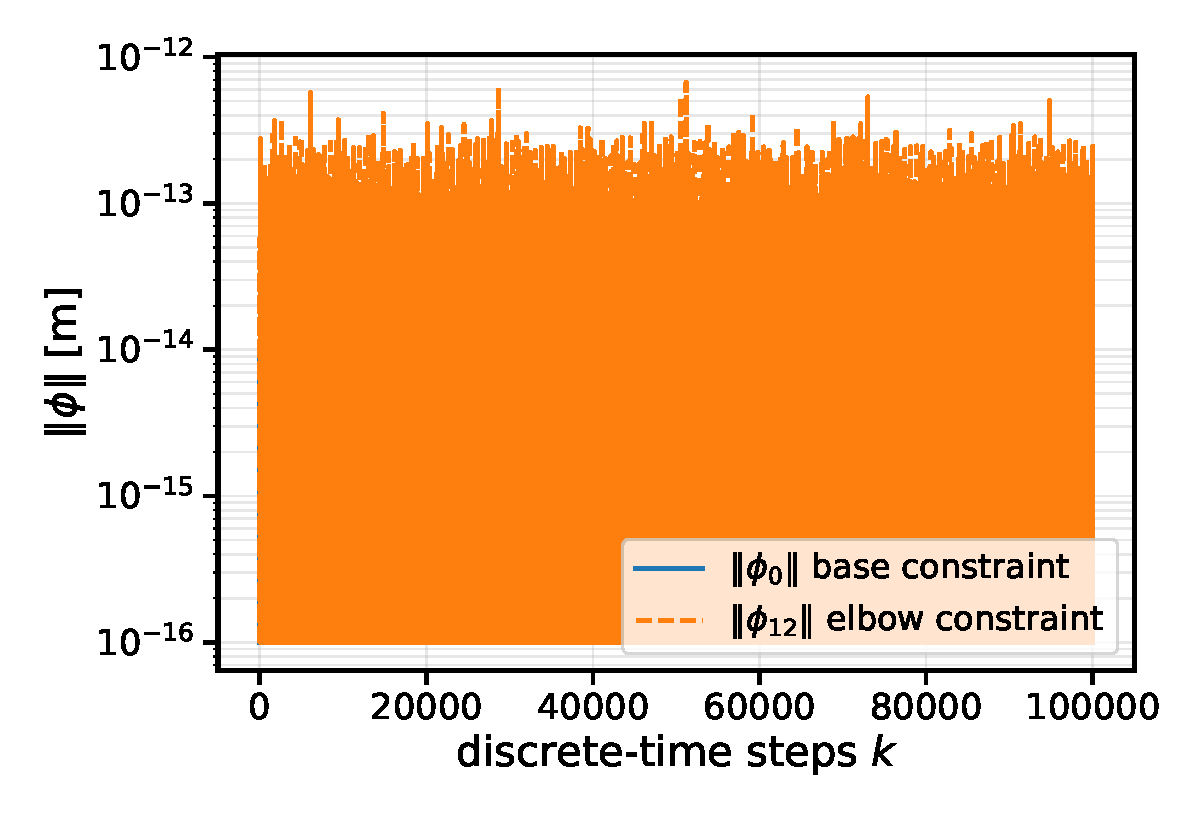
\includegraphics[width=\textwidth]{pics/Numerical_Simulation/Acrobot/acrobot_unforced_holonomic_constraint_residuals.pdf}
        \caption*{(c) Holonomic constraint residual $\phi$.}
    \end{minipage}
    \hfill
    \begin{minipage}{0.48\textwidth}
        \centering
        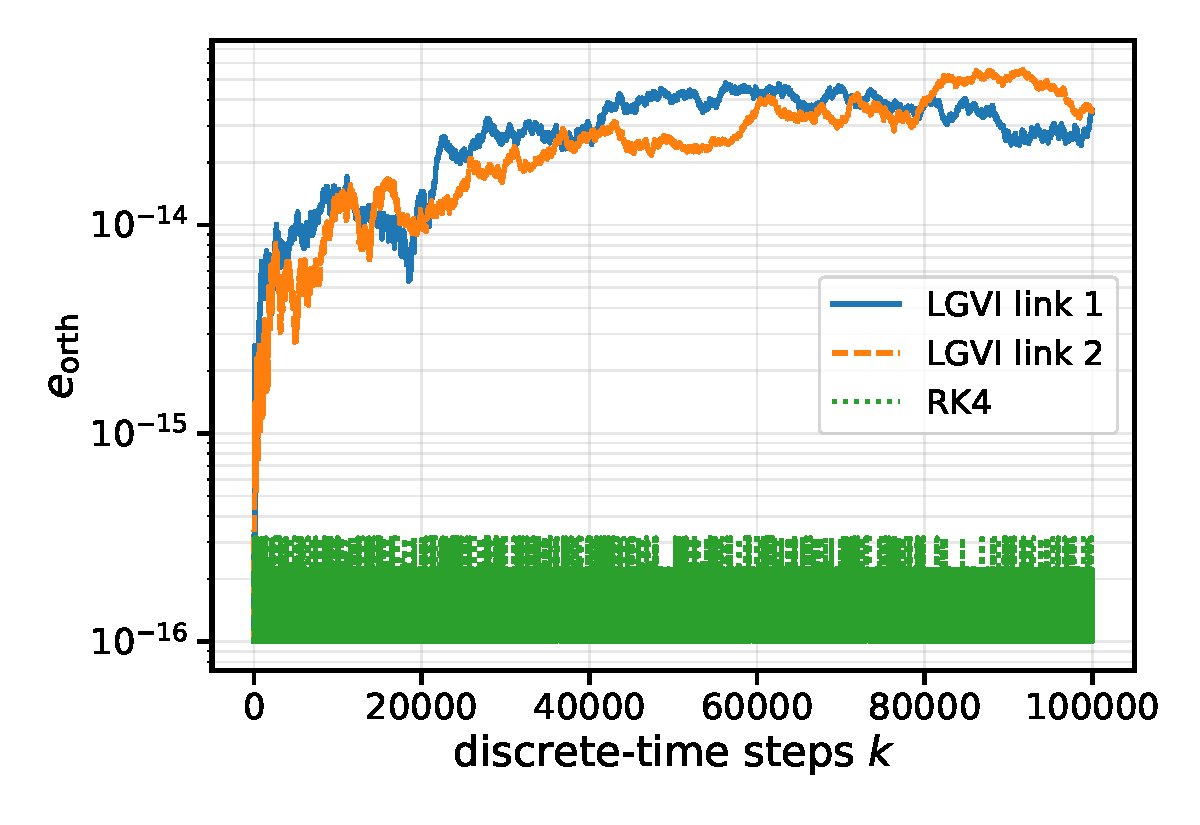
\includegraphics[width=\textwidth]{pics/Numerical_Simulation/Acrobot/acrobot_unforced_orthogonality_error.pdf}
        \caption*{(d) Orthogonality error $e_{orth}$.}
    \end{minipage}

    \caption{Comparison of the numerical preservation properties for the unforced Acrobot.}
    \label{fig:simulation_results_acrobot_unforced}
\end{figure}

\begin{figure}[t]
    \centering
    \begin{minipage}{0.48\textwidth}
        \centering
        
\includegraphics[width=\textwidth]{pics/Numerical_Simulation/Acrobot/forced_sine_total_energy.pdf}
        \caption*{(a) Total energy $E_k$.}
    \end{minipage}
    \hfill
    \begin{minipage}{0.48\textwidth}
        \centering
        
\includegraphics[width=\textwidth]{pics/Numerical_Simulation/Acrobot/forced_sine_position_error.pdf}
        \caption*{(b) Position error norm $\|\Delta \bm{x}_k \||$.}
    \end{minipage}

    \vspace{0.5em}

    \begin{minipage}{0.48\textwidth}
        \centering
        
\includegraphics[width=\textwidth]{pics/Numerical_Simulation/Acrobot/forced_sine_constraint_residuals.pdf}
        \caption*{(c) Holonomic constraint residual $\phi$.}
    \end{minipage}
    \hfill
    \begin{minipage}{0.48\textwidth}
        \centering
        
\includegraphics[width=\textwidth]{pics/Numerical_Simulation/Acrobot/forced_sine_orthogonality_error.pdf}
        \caption*{(d) Orthogonality error $e_{orth}$.}
    \end{minipage}

    \caption{Comparison of the numerical preservation properties for the controlled Acrobot.}
    \label{fig:simulation_results_acrobot_forced}
\end{figure}


\section{3D-Pendulum Optimization Results}
\label{sec:optimization_results}

SPOT-Based Implementation

Minimal Cordal Extension MD

\section{Acrobot Optimization Results}
\label{sec:acrobot_optimization_results}
Reduced Models...

\subsection{Semidefinite Optimization Results}
\label{subsec:acrobot_optimization_results}

\subsubsection{Position Reduction LGVI Model}

\subsubsection{Discretized Euler-Lagrange Model}


Tabelle 0 45 90 180 Degree SELF cliques

\subsection{Model Predictive SDP Control Results}






\begin{figure}[t]
    \centering
    \begin{minipage}{0.48\textwidth}
        \centering
        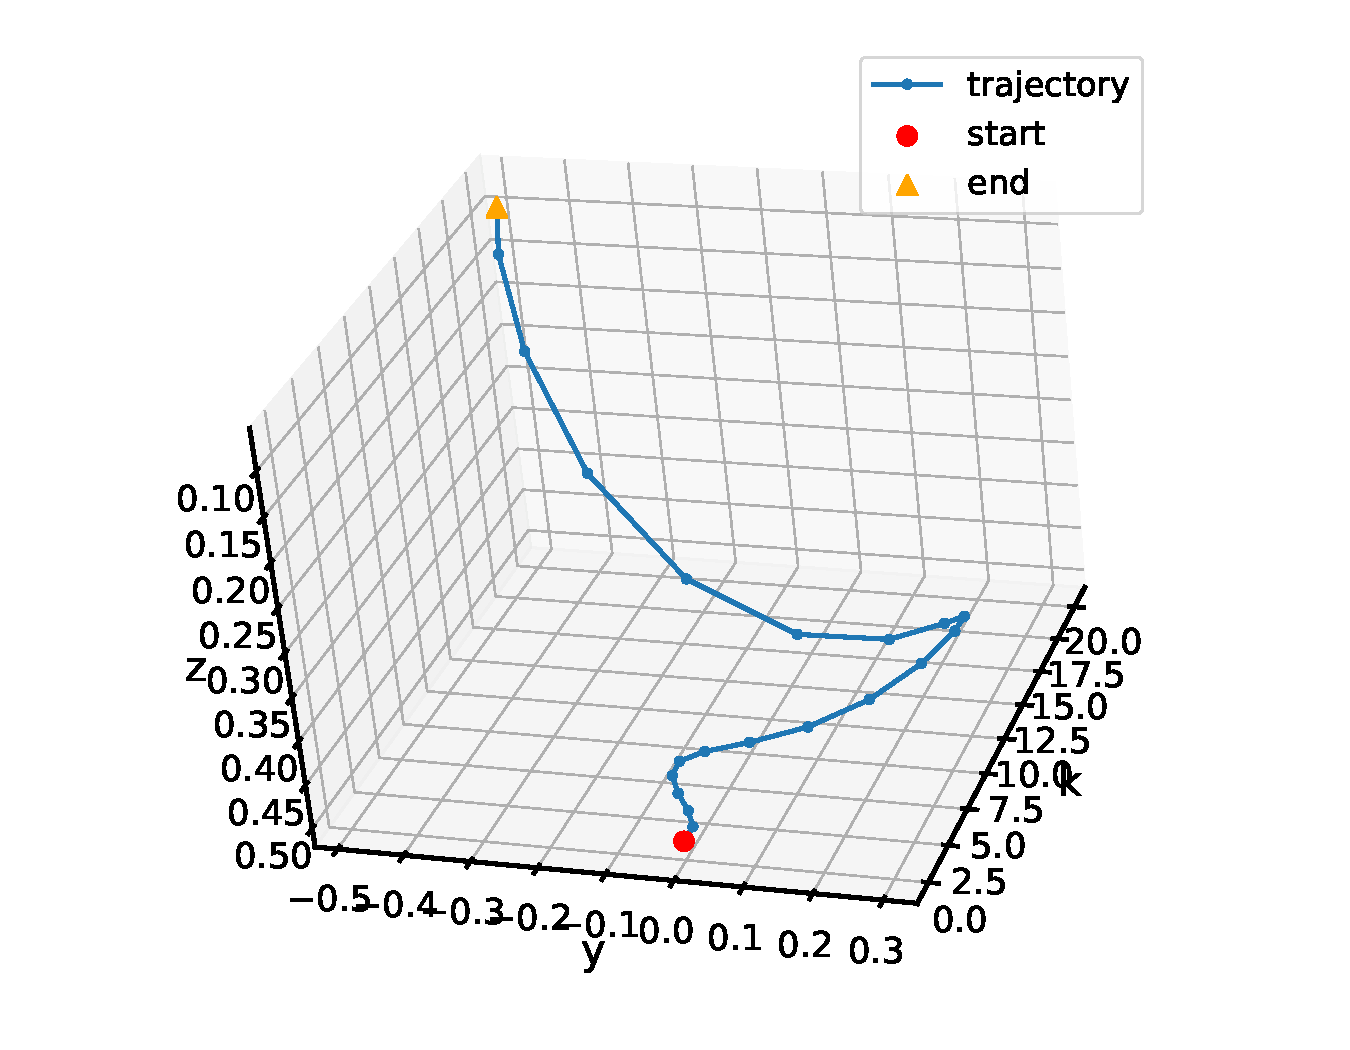
\includegraphics[width=\textwidth]{pics/Optimization/3D_Pendulum/MD_90_deg_Pendulum_trajectory.pdf}
        \caption*{(a) Center-of-mass trajectory.}
    \end{minipage}
    \hfill
    \begin{minipage}{0.48\textwidth}
        \centering
        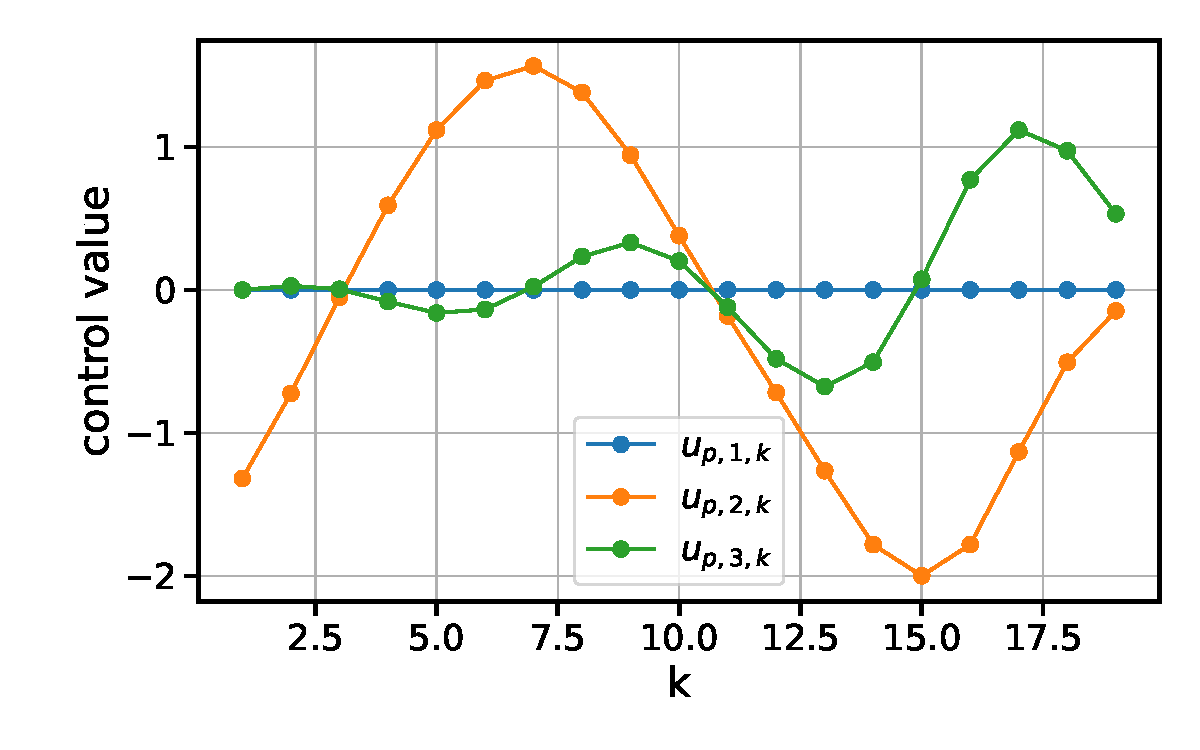
\includegraphics[width=\textwidth]{pics/Optimization/3D_Pendulum/MD_90_deg_Pendulum_control_input.pdf}
        \caption*{(b) Control inputs $\bm{u}_{p,k}$.}
    \end{minipage}

    \vspace{0.5em}

    \begin{minipage}{0.48\textwidth}
        \centering
        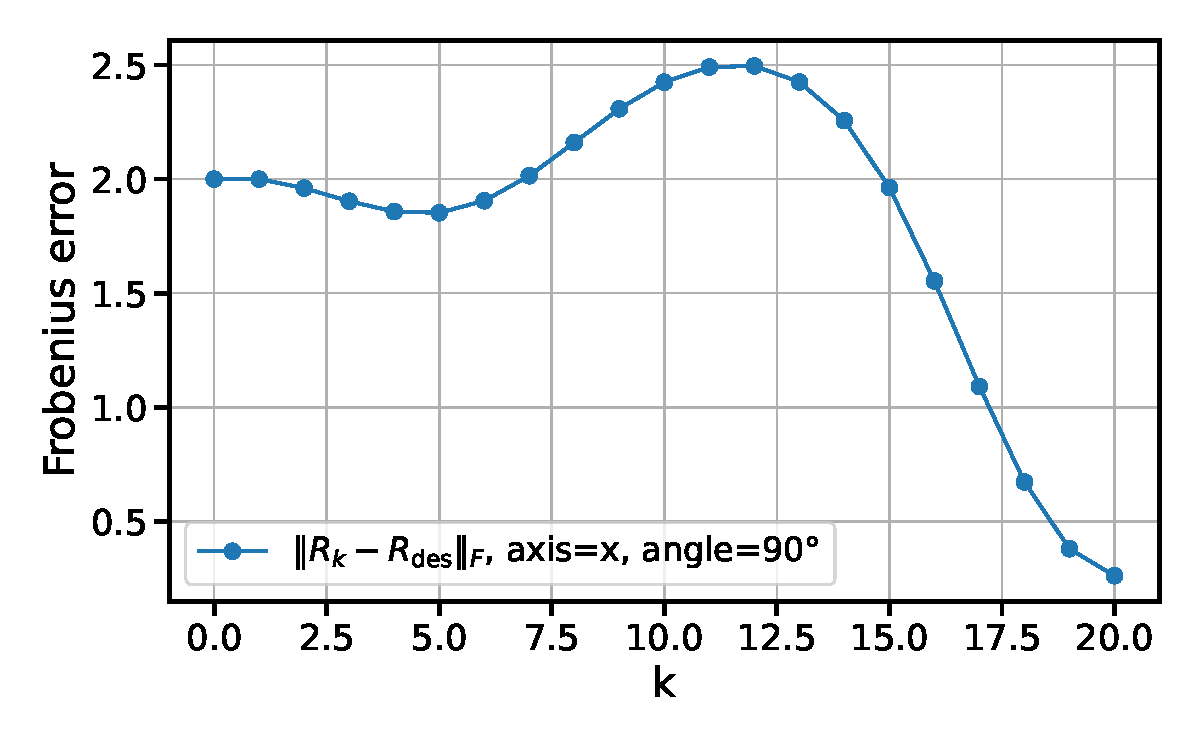
\includegraphics[width=\textwidth]{pics/Optimization/3D_Pendulum/MD_90_deg_Pendulum_frobenius.pdf}
        \caption*{(c) Frobenius tracking error $\|\bm{R}_k-\bm{R}_{\mathrm{des}}\|_F$.}
    \end{minipage}
    \hfill
    \begin{minipage}{0.48\textwidth}
        \centering
        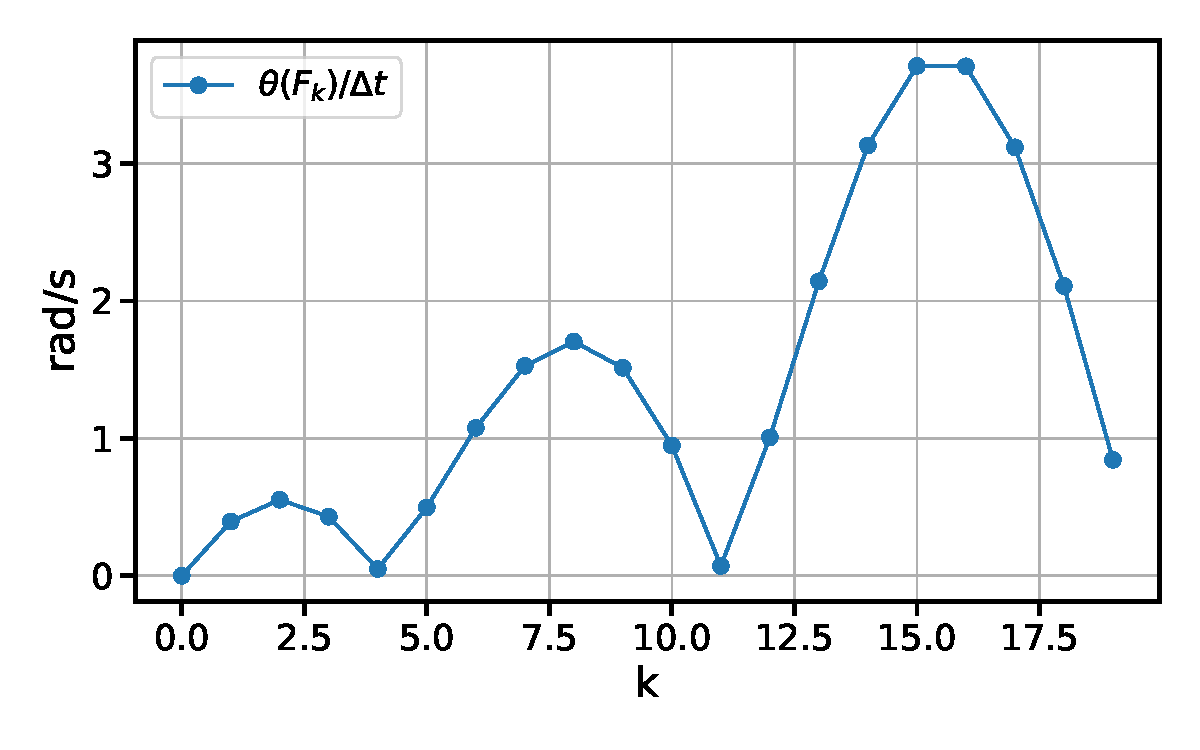
\includegraphics[width=\textwidth]{pics/Optimization/3D_Pendulum/MD_90_deg_Pendulum_F_speed.pdf}
        \caption*{(d) Relative rotation speed $\theta(\bm{F}_k)/h$.}
    \end{minipage}

    \vspace{0.5em}

    \begin{minipage}{0.48\textwidth}
        \centering
        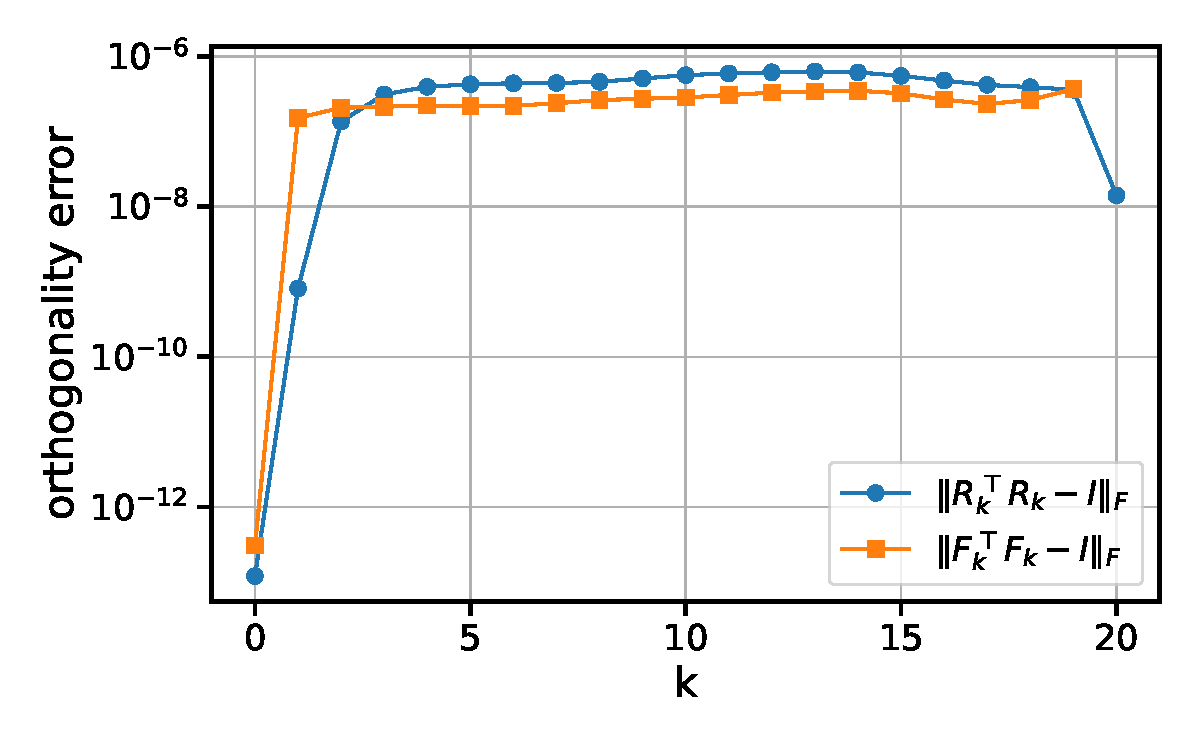
\includegraphics[width=\textwidth]{pics/Optimization/3D_Pendulum/MD_90_deg_Pendulum_orthogonality.pdf}
        \caption*{(e) Orthogonality errors of $\bm{R}_k$ and $\bm{F}_k$.}
    \end{minipage}
    \hfill
    \begin{minipage}{0.48\textwidth}
        \centering
        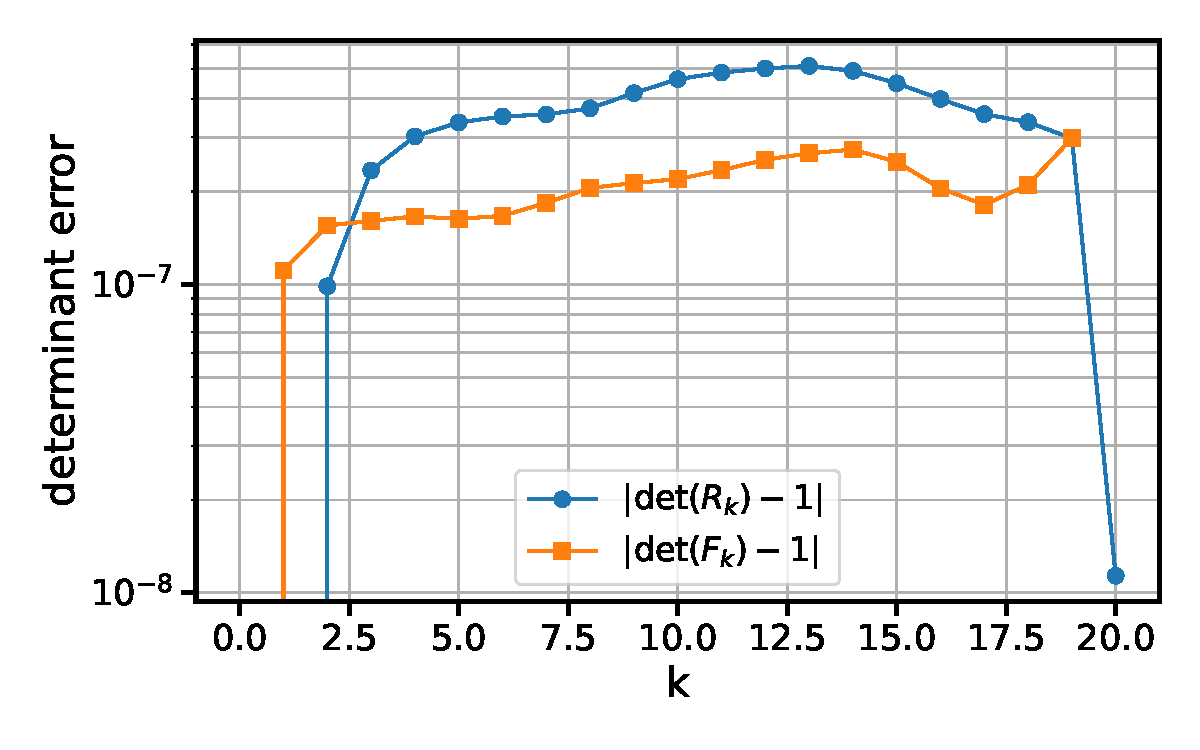
\includegraphics[width=\textwidth]{pics/Optimization/3D_Pendulum/MD_90_deg_Pendulum_determinant.pdf}
        \caption*{(f) Determinant errors of $\bm{R}_k$ and $\bm{F}_k$.}
    \end{minipage}

    \caption{SPOT optimization results for the controlled $3$D pendulum performing a $90^\circ$ rotation about the $x$-axis using the MD sparsity setting.}
    \label{fig:optimization_results_x90_md}
\end{figure}

%\begin{figure}[h]
%	\centering
%	
\includegraphics[width=1.0\textwidth]{pics/Optimization/3D_Pendulum/ordered_extraction_diagnostics_x_20.png}
%	\caption{Rotation around e1 20 degrees}
%	\label{fig:ordered_extraction}
%\end{figure}

%\subsubsection{Infulence of Sparsity Settings}
%\label{subsec:influence_sparsity_settings}

%\begin{figure}[h]
%	\centering
%	\includegraphics[width=1.0\textwidth]{}
%	\caption{}
%	\label{fig:}
%\end{figure}

%\subsubsection{Limitations}
%\label{subsec:optimization_limitations}



%\section{Experimental Results}

%A thesis almost always has an experimental part, typically some comparison to other approaches. Benchmarking takes time, for running the experiments, but also for thinking them up in the first place, and for analysing the results. Plan accordingly to spend enough time here!

%Think about what makes sense to measure, what you want to learn from your measurements. Think about what is really the relevant contribution of your thesis, and how you can prove that you have achieved your goals. Think about what you can measure in order to get a good insight into the performance of various aspects of your design, how you can distinguish between systematic and accidental effects, how you can convince yourself that your results are right. If you get surprising results, do not just say ``surprise, surprise, performance isn't as good as hoped''. Find out why. Surprises without explanation indicate either that you are clueless about what is going on, or that you have made a mistake. Unconvincing results, therefore, tend to imply unconvincing marks. 

%\paragraph{Statistics:} Measurements always have statistical (sampling) errors. Owing to the deterministic nature of simulations these are sometimes very small, as disturbing factors can be designed. However, the reader should be given an indication of how statistically significant the results are. This is done by providing at least a standard deviation in addition to averages. Whenever the results of several runs are averaged, a standard deviation can (and must) be supplied. After all, you average to reduce statistical errors.

%The reproducibility argument applies here just as much as for the implementation. Give enough detail on what you measure, and how you measure it, so that someone who has your implementation (but not your test code) or has re-done your implementation independently, should be able to repeat your measurements and arrive at essentially the same results. In some cases, results seem outright wrong in a thesis. In those cases, not enough detail is provided to allow the supervisor/reader to pinpoint the likely source of the error. Often the cause is systematic errors resulting from an incorrect measurement technique. If it seems wrong, and the text does not convince the reader that it is not wrong, the reader will assume that it is wrong.
